\documentclass[12pt,a4paper]{article}
\usepackage[margin=1in]{geometry} % 设置页面边距
\usepackage{ctex}
\usepackage{graphicx}
\usepackage{float}
\usepackage{amsmath}
\usepackage{amssymb} % 数学符号
\usepackage{booktabs} % 绘制漂亮的表格
\usepackage{array} % 数组和表格
\usepackage{multirow} % 多行合并的表格
\usepackage{caption} % 设置图片和表格的标题格式
\usepackage{subcaption} % 多个子图或表格
\usepackage{parskip}
\usepackage{forest}
\usepackage{pgfplots}
\usepackage{tikz}
\usepackage{listings}
\usetikzlibrary{patterns}
\setlength{\parindent}{0pt}

\title{\textbf{人工智能导论第三次作业}}
\author{张立博\ 2021012487}
\date{\today}

\begin{document}

\maketitle
\section{第一题\ 贝叶斯网络}
\subsection{}
\begin{gather*}
    P(-e,-s,-m,-b)\\
    =P(-e)P(-s|-e,-m)P(-m)P(-b|-m)\\
    =0.6\times0.9\times0.9\times0.9\\
    =0.4374
\end{gather*}
\subsection{}
\begin{gather*}
    P(+b)\\
    =P(+b|+m)P(+m)+P(+b|-m)P(-m)\\
    =1.0\times0.1+0.1\times0.9\\
    =0.19
\end{gather*}
\subsection{}
\begin{gather*}
    P(+m|+b)\\
    =\frac{P(+b|+m)P(+m)}{P(+b)}\\
    =\frac{1.0\times0.1}{0.19}\\
    =0.5263
\end{gather*}
\subsection{}
\begin{gather*}
    P(+m|+s,+b,+e)\\
    =\frac{P(+m,+s,+b,+e)}{P(+s,+b,+e)}\\
    =\frac{P(+m)P(+s|+e,+m)P(+b|+m)P(+e)}{P(+m,+s,+b,+e) + P(-m,+s,+b,+e)}\\
    =\frac{P(+m)P(+s|+e,+m)P(+b|+m)P(+e)}{P(+m)P(+s|+e,+m)P(+b|+m)P(+e) + P(-m)P(+s|+e,-m)P(+b|-m)P(+e)}\\
    =\frac{0.1\times1.0\times1.0\times0.4}{0.1\times1.0\times1.0\times0.4 + 0.9\times0.8\times0.1\times0.4}\\
    =0.5814
\end{gather*}
\subsection{}
在$s$未知的情况下,$m$和$e$是独立的,因此:
\begin{gather*}
    P(+e|+m)\\
    =P(+e)\\
    =0.4
\end{gather*}
\section{第二题\ 变量消除法}
\subsection{}
\begin{gather*}
    \tau _2(b,d,e,f,g) = \sum _{c}P(c|b)P(d|c)P(e|c,d)P(f|c,e)P(g|c,f)\\
\end{gather*}
剩余因子如下:
\begin{gather*}
    \tau _1(b),\tau_2(b,d,e,f,g)
\end{gather*}
\subsection{}
\begin{gather*}
    \tau_3(b,d,f,g)=\sum_{e}\tau_2(b,d,e,f,g)\\
\end{gather*}
剩余因子如下:
\begin{gather*}
    \tau _1(b),\tau_3(b,d,f,g)
\end{gather*}
\subsection{}
\begin{gather*}
    \tau_4(b,d,f)=\sum_{g}\tau_2(b,d,f,g)\\
\end{gather*}
剩余因子如下:
\begin{gather*}
    \tau _1(b),\tau_4(b,d,f)
\end{gather*}
\subsection{}
% 已知\tau_b(b),\tau_4(b,d,f),求P(B = b,D = d|F = f)
\begin{gather*}
    P(B=b,D=d|F=f)\\
    =\frac{\tau_1(b)\tau_4(b,d,f)}{\sum_{b}\tau_1(b)(\sum_{d}\tau_4(b,d,f))}\\
\end{gather*}
\subsection{}
变量消除顺序为:$A,G,E,C$\\
消除$A$后,剩余因子为:
\begin{gather*}
    \tau_1(b), P(c|b),P(d|c),P(e|c,d),P(f|c,e),P(g|c,f)
\end{gather*}
产生的新因子$\tau_1(b)$大小为1\\
消除$G$后,剩余因子为:
\begin{gather*}
    \tau_1(b), P(c|b),P(d|c),P(e|c,d),P(f|c,e),\tau_2(c,f)
\end{gather*}
产生的新因子$\tau_2(c,f)$大小为1\\
消除$E$后,剩余因子为:
\begin{gather*}
    \tau_1(b), P(c|b),P(d|c),\tau_2(c,f),\tau_3(c,d,f)
\end{gather*}
产生的新因子$\tau_3(c,d,f)$大小为2\\
消除$C$后,剩余因子为:
\begin{gather*}
    \tau_1(b),\tau_4(b,d,f)
\end{gather*}
产生的新因子$\tau_4(b,d,f)$大小为2\\
\section{第三题\ 带方差的高斯线性回归}
由已知
\begin{gather*}
    logp(D_n;w,\sigma ) = \sum_{i = 1}^{N}logp(y_n|x_n,w,\sigma )\\
    =\sum_{i = 1}^{N}log\frac{1}{\sqrt{2\pi}\sigma}exp(-\frac{(y_n-w^Tx_n)^2}{2\sigma^2})\\
    =-\frac{N}{2}log2\pi-\frac{N}{2}log\sigma^2-\frac{1}{2\sigma^2}\sum_{i = 1}^{N}(y_n-w^Tx_n)^2\\
\end{gather*}
分别对$w$和$\sigma$求导,得到
\begin{gather*}
    \frac{\partial logp(D_n;w,\sigma )}{\partial w} = \sum_{i = 1}^{N}\frac{y_n-w^Tx_n}{\sigma^2}x_n\\
    \frac{\partial logp(D_n;w,\sigma )}{\partial \sigma} = \sum_{i = 1}^{N}\frac{1}{\sigma}-\frac{(y_n-w^Tx_n)^2}{\sigma^3}\\
\end{gather*}
令导数为0,得到
\begin{gather*}
    \sum_{i = 1}^{N}\frac{y_n-w^Tx_n}{\sigma^2}x_n=0\\
    \sum_{i = 1}^{N}\frac{1}{\sigma}-\frac{(y_n-w^Tx_n)^2}{\sigma^3}=0\\
\end{gather*}
解得
\begin{gather*}
    w_{ML}=(X^TX)^{-1}X^TY\\
    \sigma_{ML}^2=\frac{1}{n}(Y-Xw_{ML})^T(Y-Xw_{ML})\\
\end{gather*}
故
\begin{gather*}
    \hat{w}=(X^TX)^{-1}X^TY\\
    \hat{\sigma} = \sqrt{\frac{1}{n}(Y-X\hat{w})^T(Y-X\hat{w})}\\
\end{gather*}
其中$x_n$为$d\times 1$的向量,$y_n$为标量,$w$为$d\times 1$的向量。\\
% 解释X,Y
$X$为$n\times d$的矩阵,$Y$为$n\times 1$的向量,$X$的第$i$行为$x_i^T$,$Y$的第$i$行为$y_i$。
\section{第四题\ 采样}
% 考虑一个在100*100网格上的采样问题。对于样本x=(x_1,x_2)属于{1,2,...,100}^2,其概率满足
% p(x_1,x_2)正比于x_1 + ln(x_1x_2+2x_1+3x_2)
% 由于样本空间非常庞大,且归一化系数难以计算,因此需要采用马尔科夫链蒙特卡洛方法进行采样。
% 假设初始状态为(2,2)
\subsection{}
\begin{gather*}
    \alpha_{ij} = min\{1,\frac{\pi_jQ_{ji}}{\pi_iQ_{ij}}\}\\
\end{gather*}
下一个状态为$(1,3)$的概率为
\begin{gather*}
    \alpha_{(2,2),(1,3)}=min\{1,\frac{p(1,3)Q}{p(2,2)Q}\}\\
    =min\{1,\frac{p(1,3)}{p(2,2)}\}\\
    =min\{1,\frac{1+ln(1\times3+2\times1+3\times3)}{2+ln(2\times2+2\times2+3\times2)}\}\\
    =min\{1,\frac{1+ln(14)}{2+ln(14)}\}\\
    =0.784
\end{gather*}
下一个状态为$(3,4)$的概率为
\begin{gather*}
    \alpha_{(2,2),(3,4)}=min\{1,\frac{p(3,4)Q}{p(2,2)Q}\}\\
    =min\{1,\frac{p(3,4)}{p(2,2)}\}\\
    =min\{1,\frac{3+ln(3\times4+2\times3+3\times4)}{2+ln(2\times2+2\times2+3\times2)}\}\\
    =min\{1,\frac{3+ln(30)}{2+ln(14)}\}\\
    =1
\end{gather*}
\subsection{}
% 使用Gibbs采样法进行采样。第一次采样过程需要采样x_1,请写出提议分布q(x_1)的形式。在此基础上,若采样到x_1=42,请写出第二次采样过程中需要采样的变量及其提议分布的形式
若初始点位于$(2,2)$,则第一次采样过程需要采样$x_1$,提议分布$q(x_1)$的形式为
\begin{gather*}
    q(x_1)=p(x_1|x_2)\\
    =\frac{p(x_1,x_2)}{p(x_2)}\\
    =\frac{x_1+ln(x_1x_2+2x_1+3x_2)}{\sum_{x_1=1}^{100}(x_1+ln(x_1x_2+2x_1+3x_2))}\\
    =\frac{x_1+ln(x_1\times2+2x_1+3\times2)}{\sum_{x_1=1}^{100}(x_1+ln(x_1\times2+2x_1+3\times2))}\\
\end{gather*}
第二次采样过程中需要采样的变量为$x_2$,若采样到$x_1 = 42$,则提议分布的形式为
\begin{gather*}
    q(x_2)=p(x_2|x_1)\\
    =\frac{p(x_1,x_2)}{p(x_1)}\\
    =\frac{42+ln(42x_2+2\times42+3x_2)}{\sum_{x_2=1}^{100}(42+ln(42x_2+2\times42+3x_2))}\\
\end{gather*}
\section{第五题\ Baum-Welch算法}
% Baum-Welch算法是EM算法的一种,其解决了隐马尔科夫模型中三大主要问题中的学习问题。HMM的学习问题可以按如下方式定义:
% 给定观测序列X={x_1,x_2,...,x_T},在隐藏序列Z={z_1,z_2,...,z_T}未知的情况下,估计模型参数\theta=(A,B,\pi)。使得在给定模型参数\theta的情况下,观测序列X出现的概率最大。
% 参数\theta = {A,B,\pi},其中A为状态转移矩阵,B为观测概率矩阵,\pi为初始状态概率向量。
% 初始概率分布\pi = (\pi_1,\pi_2,...,\pi_N),其中\pi_i = P(z_1 = s_i),i=1,2,...,N,转移矩阵A = (a_{ij}),其中a_{ij} = P(z_{t+1} = s_j|z_t = s_i),i,j=1,2,...,N,观测概率矩阵B = (b_{jk}),其中b_{jk} = P(x_t = o_k|z_t = s_j),j=1,2,...,N,k=1,2,...,M。
% 其中N为状态数,M为观测数。
\subsection{}
% 首先进行E步的计算,在这一步中我们根据当前的网络参数θ^{old}得到隐变量Z的后验概率分布q(Z) = P(Z|X,θ^{old}),然后固定q(Z),并列出ELBO得到优化目标。
% 根据ELBO写出J(\theta)
由已知:
\begin{gather*}
    q(Z) = P(Z|X,\theta^{old})\\
\end{gather*}
所以:
\begin{gather*}
    J(\theta) := L(q(Z),\theta) = \sum_{Z}q(Z)log\frac{P(X,Z|\theta)}{q(Z)}\\
    =\sum_{Z}q(Z)logP(X,Z|\theta)-\sum_{Z}q(Z)logq(Z)\\
    =\sum_{Z}P(Z|X,\theta^{old})logP(X,Z|\theta)-\sum_{Z}P(Z|X,\theta^{old})logP(Z|X,\theta^{old})\\
\end{gather*}
又因为:
\begin{gather*}
    \hat{Z} = \arg\max_{Z}P(Z|X,\theta^{old}) \propto \arg\max_{Z}P(X,Z|\theta^{old})\\
\end{gather*}
所以:
\begin{gather*}
    \arg\max_{\theta}J(\theta) = \arg\max_{\theta}\sum_{Z}P(X,Z|\theta^{old})logP(X,Z|\theta)\\
\end{gather*}
\subsection{}
% 使用模型的参数θ(包括π, A, B)来表示P(X,Z|θ),给出相应的形式
根据$HMM$的定义,可以将$P(X,Z|\theta)$表示为:
\begin{gather*}
    P(X,Z|\theta) = P(x_1,x_2,...,x_T,z_1,z_2,...,z_T|\theta)\\
\end{gather*}
根据$HMM$的独立性假设
\begin{gather*}
    P(X,Z|\theta) = P(x_1,x_2,...,x_T|z_1,z_2,...,z_T,\theta)P(z_1,z_2,...,z_T|\theta)\\
    =P(x_1,x_2,...,x_T|z_1,z_2,...,z_T,\theta)P(z_1|\theta)P(z_2|z_1,\theta)...P(z_T|z_{T-1},\theta)\\
    =P(x_1|z_1,\theta)P(x_2|z_2,\theta)...P(x_T|z_T,\theta)P(z_1|\theta)P(z_2|z_1,\theta)...P(z_T|z_{T-1},\theta)\\
\end{gather*}
其中
\begin{gather*}
    P(x_t|z_t,\theta) = b_{z_t}(x_t)\\
    P(z_t|z_{t-1},\theta) = a_{z_{t-1}z_t}\\
    P(z_1|\theta) = \pi_{z_1}\\
\end{gather*}
所以
\begin{gather*}
    P(X,Z|\theta) = \pi(z_1)B(z_1,x_1)A(z_1,z_2)B(z_2,x_2)...A(z_{T-1},z_T)B(z_T,x_T)\\
    =\pi(z_1)\prod_{t=1}^{T-1}A(z_t,z_{t+1})\prod_{t=1}^{T}B(z_t,x_t)\\
\end{gather*}
\subsection{}
令$Q(\theta, \theta^{old}) = \sum_{Z}P(X,Z|\theta^{old})logP(X,Z|\theta)$,将(2)中结果代入得到
\begin{gather*}
    Q(\theta, \theta^{old}) = \sum_{Z}P(X,Z|\theta^{old})logP(X,Z|\theta)\\
    =\sum_{Z}P(X,Z|\theta^{old})log\{\pi(z_1)\prod_{t=1}^{T-1}A(z_t,z_{t+1})\prod_{t=1}^{T}B(z_t,x_t)\}\\
    =\sum_{Z}P(X,Z|\theta^{old})log\pi(z_1)+\sum_{Z}P(X,Z|\theta^{old})\sum_{t=1}^{T-1}logA(z_t,z_{t+1})+\sum_{Z}P(X,Z|\theta^{old})\sum_{t=1}^{T}logB(z_t,x_t)\\
\end{gather*}
上式中$Q$被拆分成了三式之和,其中每一项仅与$\theta$中的一个参数有关
\subsection{}
% 上一步实现了参数之间的解耦,可以进入M步的计算,此时暂时不需要考虑\theta^{old}
% 请首先证明\sum_{Z}P(X,Z|\theta^{old})log\pi(z_1) = \sum_{i=1}^{N}P(X,z_1 = i|\theta^{old})log\pi_i
证:
\begin{gather*}
    \sum_{Z}P(X,Z|\theta^{old})\log\pi(z_1)\\
    = \sum_{z_1=1}^{N}\sum_{z_2,...,z_T}P(X,z_1,z_2,...,z_T|\theta^{old})\log\pi(z_1)\\
    =\sum_{z_1=1}^{N}P(X,z_1|\theta^{old})\sum_{z_2,...,z_T}P(z_2,...,z_T|X,z_1,\theta^{old})\log\pi(z_1)\\
    = \sum_{z_1=1}^{N}P(X,z_1|\theta^{old})\log\pi(z_1)\sum_{z_2,...,z_T}P(z_2,...,z_T|X,z_1,\theta^{old})\\
\end{gather*}
由于内部求和符号中的条件概率 $P(z_2,...,z_T|X,z_1,\theta^{old})$ 是对给定的 $z_1$ 条件下后续的隐藏状态的概率,根据概率的归一性,有:
\begin{gather*}
    \sum_{z_2,...,z_T}P(z_2,...,z_T|X,z_1,\theta^{old}) = 1\\
\end{gather*}
所以
\begin{gather*}
    \sum_{Z}P(X,Z|\theta^{old})log\pi(z_1)\\
    = \sum_{z_1=1}^{N}P(X,z_1|\theta^{old})\log\pi(z_1)\\
    = \sum_{i=1}^{N}P(X,z_1 = i|\theta^{old})\log\pi_i\\
\end{gather*}
使用拉格朗日乘子法,求$\sum_{Z}P(X,Z|\theta^{old})\log\pi_{z_1}$在$\sum_{i=1}^{N}\pi_i = 1$下取到极大值时$\pi_i$的值\\
首先定义拉格朗日函数:
\begin{gather*}
    L(\pi,\lambda) = \sum_{i=1}^{N}P(X,z_1 = i|\theta^{old})\log\pi_i + \lambda(\sum_{i=1}^{N}\pi_i - 1)\\
\end{gather*}
题目要求$\sum_{Z}P(X,Z|\theta^{old})\log\pi_{z_1}$在$\sum_{i=1}^{N}\pi_i = 1$下取到极大值,即找到使得拉格朗日函数取到极大值的$\pi_i$的值\\
对拉格朗日函数求偏导并令其为0。\\
首先对$\pi_i$求偏导:
\begin{gather*}
    \frac{\partial L(\pi,\lambda)}{\partial \pi_i} = \frac{P(X,z_1 = i|\theta^{old})}{\pi_i} + \lambda = 0\\
\end{gather*}
然后对$\lambda$求偏导:
\begin{gather*}
    \frac{\partial L(\pi,\lambda)}{\partial \lambda} = \sum_{i=1}^{N}\pi_i - 1 = 0\\
\end{gather*}
联立求解得到:
\begin{gather*}
    \pi_i = -\frac{P(X,z_1 = i|\theta^{old})}{\lambda}\\
    \sum_{i=1}^{N}\pi_i = -\frac{\sum_{i=1}^{N}P(X,z_1 = i|\theta^{old})}{\lambda} = 1\\
    \lambda = -\sum_{i=1}^{N}P(X,z_1 = i|\theta^{old})\\
    \pi_i = \frac{P(X,z_1 = i|\theta^{old})}{\sum_{i=1}^{N}P(X,z_1 = i|\theta^{old})}\\
\end{gather*}
\subsection{}
求解$Q(\theta,\theta^{old})$取极大值时$a_{ij}$和$b_{j}(k)$的取值\\
求解过程与上一小题类似,首先证明:
\begin{gather}
    \sum_{Z}P(X,Z|\theta^{old})\sum_{t=1}^{T-1}logA(z_t,z_{t+1}) = \sum_{i=1}^{N}\sum_{j=1}^{N}\sum_{t=1}^{T-1}P(X,z_t = i,z_{t+1} = j|\theta^{old})loga_{ij}
\end{gather}
证:
\begin{gather*}
    \sum_{Z}P(X,Z|\theta^{old})\sum_{t=1}^{T-1}logA(z_t,z_{t+1})\\
    = \sum_{z_1=1}^{N}\sum_{z_2,...,z_T}P(X,z_1,z_2,...,z_T|\theta^{old})\sum_{t=1}^{T-1}logA(z_t,z_{t+1})\\
    =\sum_{z_1=1}^{N}P(X,z_1|\theta^{old})\sum_{z_2,...,z_T}P(z_2,...,z_T|X,z_1,\theta^{old})\sum_{t=1}^{T-1}logA(z_t,z_{t+1})\\
    = \sum_{z_1=1}^{N}P(X,z_1|\theta^{old})\sum_{z_2,...,z_T}P(z_2,...,z_T|X,z_1,\theta^{old})\sum_{t=1}^{T-1}loga_{z_tz_{t+1}}\\
    = \sum_{z_1=1}^{N}P(X,z_1|\theta^{old})\sum_{z_2,...,z_T}P(z_2,...,z_T|X,z_1,\theta^{old})\sum_{i=1}^{N}\sum_{j=1}^{N}\sum_{t=1}^{T-1}I(z_t = i,z_{t+1} = j)loga_{ij}\\
    = \sum_{i=1}^{N}\sum_{j=1}^{N}\sum_{t=1}^{T-1}\sum_{z_1=1}^{N}P(X,z_1|\theta^{old})P(z_2,...,z_T|X,z_1,\theta^{old})I(z_t = i,z_{t+1} = j)loga_{ij}\\
    = \sum_{i=1}^{N}\sum_{j=1}^{N}\sum_{t=1}^{T-1}P(X,z_t = i,z_{t
    +1} = j|\theta^{old})loga_{ij}\\
\end{gather*}
使用拉格朗日乘子法,求$\sum_{Z}P(X,Z|\theta^{old})\sum_{t=1}^{T-1}logA(z_t,z_{t+1})$在$\sum_{j=1}^{N}a_{ij} = 1$下取到极大值时$a_{ij}$的值\\
首先定义拉格朗日函数:
\begin{gather*}
    L(A,\lambda) = \sum_{i=1}^{N}\sum_{j=1}^{N}\sum_{t=1}^{T-1}P(X,z_t = i,z_{t+1} = j|\theta^{old})loga_{ij} + \lambda(\sum_{j=1}^{N}a_{ij} - 1)\\
\end{gather*}
题目要求$\sum_{Z}P(X,Z|\theta^{old})\sum_{t=1}^{T-1}logA(z_t,z_{t+1})$在$\sum_{j=1}^{N}a_{ij} = 1$下取到极大值,即找到使得拉格朗日函数取到极大值的$a_{ij}$的值\\
对拉格朗日函数求偏导并令其为0。\\
首先对$a_{ij}$求偏导:
\begin{gather*}
    \frac{\partial L(A,\lambda)}{\partial a_{ij}} = \frac{\sum_{t=1}^{T-1}P(X,z_t = i,z_{t+1} = j|\theta^{old})}{a_{ij}} + \lambda = 0\\
\end{gather*}
然后对$\lambda$求偏导:
\begin{gather*}
    \frac{\partial L(A,\lambda)}{\partial \lambda} = \sum_{j=1}^{N}a_{ij} - 1 = 0\\
\end{gather*}
联立求解得到:
\begin{gather*}
    a_{ij} = -\frac{\sum_{t=1}^{T-1}P(X,z_t = i,z_{t+1} = j|\theta^{old})}{\lambda}\\
    \sum_{j=1}^{N}a_{ij} = -\frac{\sum_{j=1}^{N}\sum_{t=1}^{T-1}P(X,z_t = i,z_{t+1} = j|\theta^{old})}{\lambda} = 1\\
    \lambda = -\sum_{j=1}^{N}\sum_{t=1}^{T-1}P(X,z_t = i,z_{t+1} = j|\theta^{old})\\
    a_{ij} = \frac{\sum_{t=1}^{T-1}P(X,z_t = i,z_{t+1} = j|\theta^{old})}{\sum_{j=1}^{N}\sum_{t=1}^{T-1}P(X,z_t = i,z_{t+1} = j|\theta^{old})}\\
\end{gather*}
接着证明:
\begin{gather}
    \sum_{Z}P(X,Z|\theta^{old})\sum_{t=1}^{T}logB(z_t,x_t) = \sum_{j=1}^{N}\sum_{k=1}^{M}\sum_{t=1}^{T}P(X,z_t = j,x_t = k|\theta^{old})logb_{j}(k)
\end{gather}
证:
\begin{gather*}
    \sum_{Z}P(X,Z|\theta^{old})\sum_{t=1}^{T}logB(z_t,x_t)\\
    = \sum_{z_1=1}^{N}\sum_{z_2,...,z_T}P(X,z_1,z_2,...,z_T|\theta^{old})\sum_{t=1}^{T}logB(z_t,x_t)\\
    =\sum_{z_1=1}^{N}P(X,z_1|\theta^{old})\sum_{z_2,...,z_T}P(z_2,...,z_T|X,z_1,\theta^{old})\sum_{t=1}^{T}logB(z_t,x_t)\\
    = \sum_{z_1=1}^{N}P(X,z_1|\theta^{old})\sum_{z_2,...,z_T}P(z_2,...,z_T|X,z_1,\theta^{old})\sum_{t=1}^{T}logb_{z_t}(x_t)\\
    = \sum_{z_1=1}^{N}P(X,z_1|\theta^{old})\sum_{z_2,...,z_T}P(z_2,...,z_T|X,z_1,\theta^{old})\sum_{j=1}^{N}\sum_{k=1}^{M}\sum_{t=1}^{T}I(z_t = j,x_t = k)logb_{j}(k)\\
    = \sum_{j=1}^{N}\sum_{k=1}^{M}\sum_{t=1}^{T}\sum_{z_1=1}^{N}P(X,z_1|\theta^{old})P(z_2,...,z_T|X,z_1,\theta^{old})I(z_t = j,x_t = k)logb_{j}(k)\\
    = \sum_{j=1}^{N}\sum_{k=1}^{M}\sum_{t=1}^{T}P(X,z_t = j,x_t = k|\theta^{old})logb_{j}(k)\\
\end{gather*}
使用拉格朗日乘子法,求$\sum_{Z}P(X,Z|\theta^{old})\sum_{t=1}^{T}logB(z_t,x_t)$在$\sum_{k=1}^{M}b_{j}(k) = 1$下取到极大值时$b_{j}(k)$的值\\
首先定义拉格朗日函数:
\begin{gather*}
    L(B,\lambda) = \sum_{j=1}^{N}\sum_{k=1}^{M}\sum_{t=1}^{T}P(X,z_t = j,x_t = k|\theta^{old})logb_{j}(k) + \lambda(\sum_{k=1}^{M}b_{j}(k) - 1)\\
\end{gather*}
题目要求$\sum_{Z}P(X,Z|\theta^{old})\sum_{t=1}^{T}logB(z_t,x_t)$在$\sum_{k=1}^{M}b_{j}(k) = 1$下取到极大值,即找到使得拉格朗日函数取到极大值的$b_{j}(k)$的值\\
对拉格朗日函数求偏导并令其为0。\\
首先对$b_{j}(k)$求偏导:
\begin{gather*}
    \frac{\partial L(B,\lambda)}{\partial b_{j}(k)} = \frac{\sum_{t=1}^{T}P(X,z_t = j,x_t = k|\theta^{old})}{b_{j}(k)} + \lambda = 0\\
\end{gather*}
然后对$\lambda$求偏导:
\begin{gather*}
    \frac{\partial L(B,\lambda)}{\partial \lambda} = \sum_{k=1}^{M}b_{j}(k) - 1 = 0\\
\end{gather*}
联立求解得到:
\begin{gather*}
    b_{j}(k) = -\frac{\sum_{t=1}^{T}P(X,z_t = j,x_t = k|\theta^{old})}{\lambda}\\
    \sum_{k=1}^{M}b_{j}(k) = -\frac{\sum_{k=1}^{M}\sum_{t=1}^{T}P(X,z_t = j,x_t = k|\theta^{old})}{\lambda} = 1\\
    \lambda = -\sum_{k=1}^{M}\sum_{t=1}^{T}P(X,z_t = j,x_t = k|\theta^{old})\\
    b_{j}(k) = \frac{\sum_{t=1}^{T}P(X,z_t = j,x_t = k|\theta^{old})}{\sum_{k=1}^{M}\sum_{t=1}^{T}P(X,z_t = j,x_t = k|\theta^{old})}\\
\end{gather*}
\subsection{}
由已知
\begin{gather*}
    \gamma_{t}^{old}(i) = P(z_t = i|X,\theta^{old})\\
    \xi_{t}^{old}(i,j) = P(z_t = i,z_{t+1} = j|X,\theta^{old})\\
\end{gather*}
使用课上讲过的前向-后向算法,对于给定参数$\theta^{old}$的HMM,可以求出:
\begin{gather*}
    \alpha_{t}^{old}(i) = P(z_t = i|x_1,x_2,...,x_t,\theta^{old})\\
    \beta_{t}^{old}(i) = P(x_{t+1},x_{t+2},...,x_T|z_t = i,\theta^{old})\\
\end{gather*}
下面使用$\alpha_t^{old}(i),\beta_t^{old}(i),a_{ij}^{old},b_j^{old}{(k)}$表示出$\gamma_{t}^{old}(i),\xi_{t}^{old}(i,j)$\\
首先表示出$\gamma_{t}^{old}(i)$:\\
\begin{gather*}
    \gamma_{t}^{old}(i) = P(z_t = i|X,\theta^{old})\\
    = \frac{P(z_t = i,X|\theta^{old})}{P(X|\theta^{old})}\\
    = \frac{P(z_t = i,x_1,x_2,...,x_T|\theta^{old})}{P(X|\theta^{old})}\\
    = \frac{P(z_t = i,x_1,x_2,...,x_t,x_{t+1},...,x_T|\theta^{old})}{P(X|\theta^{old})}\\
    = \frac{P(z_t = i,x_1,x_2,...,x_t|\theta^{old})P(x_{t+1},...,x_T|z_t = i,\theta^{old})}{P(X|\theta^{old})}\\
    = \frac{P(z_t = i,x_1,x_2,...,x_t|\theta^{old})P(x_{t+1},...,x_T|z_t = i,\theta^{old})}{\sum_{j=1}^{N}P(z_t = j,x_1,x_2,...,x_t|\theta^{old})P(x_{t+1},...,x_T|z_t = j,\theta^{old})}\\
    = \frac{\alpha_{t}^{old}(i)\beta_{t}^{old}(i)}{\sum_{j=1}^{N}\alpha_{t}^{old}(j)\beta_{t}^{old}(j)}\\
\end{gather*}
然后表示出$\xi_{t}^{old}(i,j)$:\\
\begin{gather*}
    \xi_{t}^{old}(i,j) = P(z_t = i,z_{t+1} = j|X,\theta^{old})\\
    = \frac{P(z_t = i,z_{t+1} = j,X|\theta^{old})}{P(X|\theta^{old})}\\
    = \frac{P(z_t = i,z_{t+1} = j,x_1,x_2,...,x_T|\theta^{old})}{P(X|\theta^{old})}\\
    = \frac{P(z_t = i,z_{t+1} = j,x_1,x_2,...,x_t,x_{t+1},...,x_T|\theta^{old})}{P(X|\theta^{old})}\\
    = \frac{P(z_t = i,z_{t+1} = j,x_1,x_2,...,x_t|\theta^{old})P(x_{t+1},...,x_T|z_t = i,z_{t+1} = j,\theta^{old})}{P(X|\theta^{old})}\\
    = \frac{P(z_t = i,x_1,x_2,...,x_t|\theta^{old})P(z_{t+1} = j|x_1,x_2,...,x_t,z_t = i,\theta^{old})P(x_{t+1},...,x_T|z_t = i,z_{t+1} = j,\theta^{old})}{P(X|\theta^{old})}\\
    = \frac{P(z_t = i,x_1,x_2,...,x_t|\theta^{old})P(z_{t+1} = j|x_1,x_2,...,x_t,z_t = i,\theta^{old})P(x_{t+1},...,x_T|z_{t+1} = j,\theta^{old})}{P(X|\theta^{old})}\\
    = \frac{P(z_t = i,x_1,x_2,...,x_t|\theta^{old})P(z_{t+1} = j|x_1,x_2,...,x_t,z_t = i,\theta^{old})P(x_{t+1},...,x_T|z_{t+1} = j,\theta^{old})}{\sum
    _{i=1}^{N}\sum_{j=1}^{N}P(z_t = i,z_{t+1} = j,x_1,x_2,...,x_t|\theta^{old})P(x_{t+1},...,x_T|z_t = i,z_{t+1} = j,\theta^{old})}\\
    = \frac{\alpha_{t}^{old}(i)a_{ij}^{old}b_j^{old}(x_{t+1})\beta_{t+1}^{old}(j)}{\sum_{i=1}^{N}\sum_{j=1}^{N}\alpha_{t}^{old}(i)a_{ij}^{old}b_j^{old}(x_{t+1})\beta_{t+1}^{old}(j)}\\
\end{gather*}
\subsection{}
回顾5.4和5.5的结果,使用$\gamma_{t}^{old}(i),\xi_{t}^{old}(i,j)$表示出$\pi_i,a_{ij},b_j(k)$\\
首先表示出$\pi_i$:\\
\begin{gather*}
    \pi_i = \frac{P(z_1 = i|X,\theta^{old})}{P(X|\theta^{old})}\\
    = \frac{P(z_1 = i,X|\theta^{old})}{P(X|\theta^{old})}\\
    = \frac{P(z_1 = i,x_1,x_2,...,x_T|\theta^{old})}{P(X|\theta^{old})}\\
    = \frac{P(z_1 = i,x_1,x_2,...,x_T|\theta^{old})}{\sum_{j=1}^{N}P(z_1 = j,x_1,x_2,...,x_T|\theta^{old})}\\
    = \frac{\sum_{t=1}^{T}P(X,z_1 = i,x_1,x_2,...,x_T|\theta^{old})}{\sum_{j=1}^{N}\sum_{t=1}^{T}P(X,z_1 = j,x_1,x_2,...,x_T|\theta^{old})}\\
    = \frac{\sum_{t=1}^{T}\gamma_{t}^{old}(i)}{\sum_{j=1}^{N}\sum_{t=1}^{T}\gamma_{t}^{old}(j)}\\
\end{gather*}
然后表示出$a_{ij}$:\\
\begin{gather*}
    a_{ij} = \frac{P(z_t = i,z_{t+1} = j|X,\theta^{old})}{P(X|\theta^{old})}\\
    = \frac{P(z_t = i,z_{t+1} = j,x_1,x_2,...,x_T|\theta^{old})}{P(X|\theta^{old})}\\
    = \frac{P(z_t = i,z_{t+1} = j,x_1,x_2,...,x_T|\theta^{old})}{\sum_{i=1}^{N}\sum_{j=1}^{N}P(z_t = i,z_{t+1} = j,x_1,x_2,...,x_T|\theta^{old})}\\
    = \frac{\sum_{t=1}^{T-1}P(X,z_t = i,z_{t+1} = j|\theta^{old})}{\sum_{i=1}^{N}\sum_{j=1}^{N}\sum_{t=1}^{T-1}P(X,z_t = i,z_{t+1} = j|\theta^{old})}\\
    = \frac{\sum_{t=1}^{T-1}\xi_{t}^{old}(i,j)}{\sum_{i=1}^{N}\sum_{j=1}^{N}\sum_{t=1}^{T-1}\xi_{t}^{old}(i,j)}\\
\end{gather*}
最后表示出$b_j(k)$:\\
\begin{gather*}
    b_j(k) = \frac{P(x_t = k|z_t = j,X,\theta^{old})}{P(X|\theta^{old})}\\
    = \frac{P(x_t = k,z_t = j,X|\theta^{old})}{P(X|\theta^{old})}\\
    = \frac{P(x_t = k,z_t = j,X|\theta^{old})}{\sum_{j=1}^{N}P(x_t = k,z_t = j,X|\theta^{old})}\\
    = \frac{\sum_{t=1}^{T}P(X,z_t = j,x_t = k|\theta^{old})}{\sum_{j=1}^{N}\sum_{t=1}^{T}P(X,z_t = j,x_t = k|\theta^{old})}\\
    = \frac{\sum_{t=1}^{T}\gamma_{t}^{old}(j)I(x_t = k)}{\sum_{j=1}^{N}\sum_{t=1}^{T}\gamma_{t}^{old}(j)}\\
\end{gather*}
结合上述推理过程,Baum-Welch算法的伪代码如下:\\
% 用文字给出Baum-Welch算法的伪代码
\textbf{重复直到收敛:}\\
\quad \textbf{E步:}\\
\quad \quad 使用前向-后向算法计算$\alpha_{t}^{old}(i),\beta_{t}^{old}(i)$\\
\quad \quad 使用$\alpha_t^{old}(i),\beta_t^{old}(i),a_{ij}^{old},b_j^{old}{(k)}$表示出$\gamma_{t}^{old}(i),\xi_{t}^{old}(i,j)$\\
\quad \textbf{M步:}\\
\quad \quad 使用$\gamma_{t}^{old}(i),\xi_{t}^{old}(i,j)$表示出$\pi_i,a_{ij},b_j(k)$\\
\quad \quad 使用$\pi_i,a_{ij},b_j(k)$更新模型参数$\theta$\\
\quad \quad 使用更新后的模型参数$\theta$计算$Q(\theta,\theta^{old})$\\
\quad \quad 计算$Q(\theta,\theta^{old})$的相对变化$\delta$\\
\quad \quad 更新$\theta^{old}$为$\theta$\\
\textbf{输出:}模型参数$\theta$
\section{第六题\ LDA}
\subsection{}
Variational EM LDA的伪代码如下:
\begin{lstlisting}[language=Python, numbers = left, escapechar=|]
    预处理数据集,得到docs和vocab
    初始化lda部分模型参数:K(主题数),V(词汇表大小),alpha(超参数)
    对给定的文档集合进行模型拟合:
        初始化监测收敛性的变量prev_bound(inf),delta(-inf),D(文档数)
        根据数据初始化模型参数:
            使用随机选择的文档子集的词频计数初始化每个主题
            通过最大似然估计计算主题-词分布的对数矩阵log_betas(V,K)
            初始化主题-文档分布矩阵gammas(D,K)
            # 重复优化参数直到收敛
            for i in range(max_epochs):
                更新参数并计算bound的值
                计算bound的相对变化delta
                打印进度
                更新prev_bound为当前bound
                检查是否收敛:若是则停止迭代
                如果vocab不为空且选择展示主题:输出每个主题的高频词
\end{lstlisting}
\subsection{}
完整代码见附件\textbf{main.py}
\subsection{}
设置不同的K,得到的结果如下:
\begin{figure}[H]
    \centering
    
\includegraphics[width=0.8\textwidth]{5_.jpg}
    \caption{K=5}
\end{figure}
\begin{figure}[H]
    \centering
    
\includegraphics[width=0.8\textwidth]{10_.jpg}
    \caption{K=10}
\end{figure}
\begin{figure}[H]
    \centering
    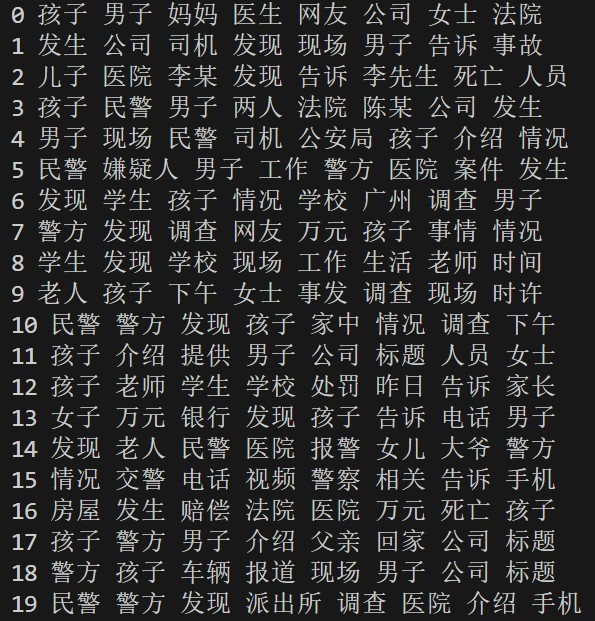
\includegraphics[width=0.8\textwidth]{20_.jpg}
    \caption{K=15}
\end{figure}
\subsection{}
观察结果发现,分类效果最好的是K=10的情况,效果比较明显的主题如:
\begin{enumerate}
    \item 主题0:男子\ 警方\ 民警\ 发现\ 现场\ 人员\ 发生\ 报警
    \item 主题5:父亲\ 手机\ 发生\ 母亲\ 生活\ 孩子\ 妈妈\ 事情
\end{enumerate}
可能的原因如下:
\begin{enumerate}
    \item K=5时,每个主题的词汇量较大,负责解释更多的数据变化,这可能导致模型欠拟合,无法捕捉数据中的复杂结构,分类效果较差
    \item K=15时,每个主题的词汇量较小,可能导致模型过拟合,将噪声也作为主题进行建模,影响分类效果,分类效果较差
    \item K=10时,每个主题的词汇量适中,适当地平衡了模型的复杂性和表达能力方面,分类效果较好
\end{enumerate}
\end{document}